\subsection{Artificial Neural Network}
When we fit our data to a ANN model with one hidden unit, it had an error rate that kept being around 34\%. This we were able to decrease, by increasing the number of k folds and how many hidden units we had, but this could result in over fitting. Here it would properly be around k folds 10 with 25-50 hidden units maybe it would had been better with more, but because of computation time we could not check those out. This also makes some sense, since we have 462 inputs and the best number of hidden units usually lies between the number of inputs and outputs but if hidden units is placed to high it might overfit.
\begin{table}[H]
\begin{longtable}{ccccccc}
\hline 
   & 1 			 & 5 		   & 7 			 & 10		   & 25			 & 50 \\ \hline
5  & 34.623656\% & 34.406265\% & 33.316971\% & 33.328658\% & 30.299205\% & 22.059374\% \\ 
10 & 34.583719\% & 34.204440\% & 34.181314\% & 31.359852\% & 30.083256\% & 21.221092\% \\ \hline 
\end{longtable}
\end{table}
Below you can see the 2 learning curves for 25 and 50 hidden units, with 10 k fold, where you are able to see the numbers of epochs (steps in training process) and how large an error rate were found during the computation.
\begin{figure}[H]
\centering
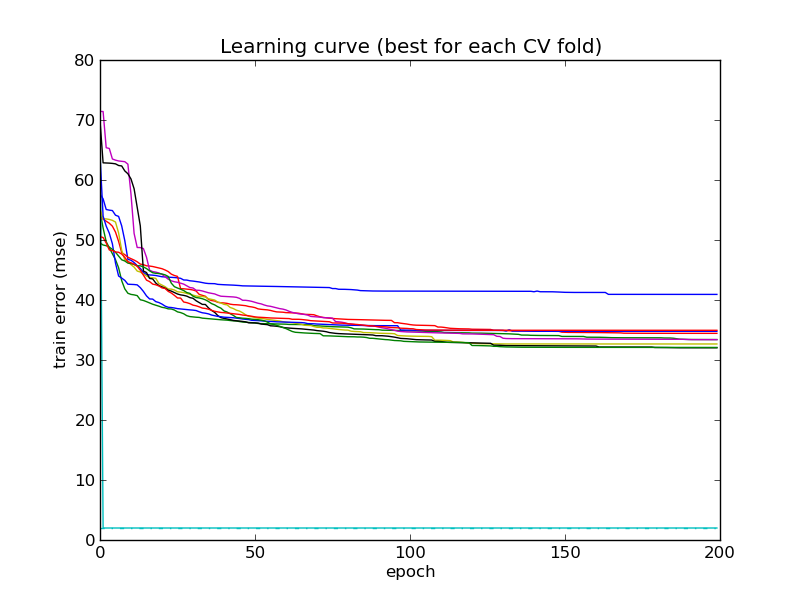
\includegraphics[width=7.5cm, keepaspectratio=true]{pictures/ann_1_10_25.png}
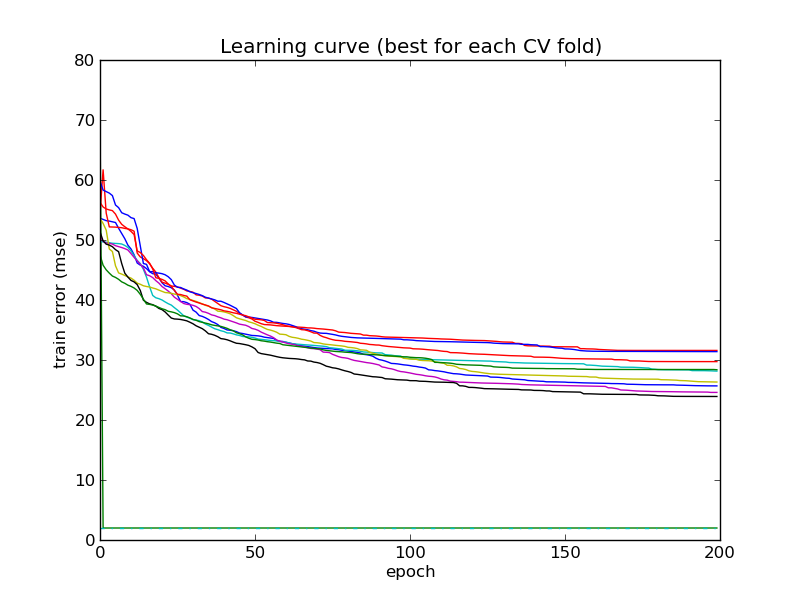
\includegraphics[width=7.5cm, keepaspectratio=true]{pictures/ann_1_10_50.png}
\vspace{-0.4cm}
\caption{\footnotesize 25 hidden vs. 50 hidden on a 10 k fold}
\label{full_10_25_50}
\end{figure}
When we then try to compute the learning curve when we have taken the 4 least important attributes out then we will get something like figure \ref{notfull_10_25_50}. This specific graph has an error rate on 24,25\%, which is a bit higher then the error rate for ANN model for all the attributes. But it is close enough so we can say it shows the same.
\begin{figure}[H]
\centering
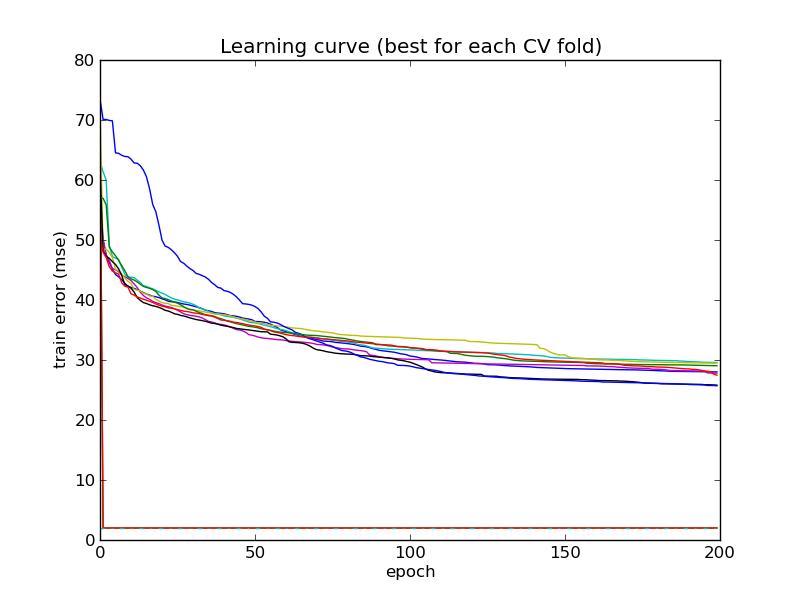
\includegraphics[width=7.5cm, keepaspectratio=true]{pictures/figure_1.png}
\vspace{-0.4cm}
\caption{\footnotesize 50 hidden on a 10 k fold with the 4 least important attributes taken out}
\label{notfull_10_25_50}
\end{figure}
When we then are trying to fit the 2 principle components with the most influence in a ANN model then we are able 2 plot it in a 2d graph, and are able to see how well it actually fit. Since we now have the same numbers of input 462. This time we only have 4 outputs because we needed enough space to fit the output graphs. Figure \ref{ann} shows how well the 2 pc fits with 230 hidden units. You can see in the left lower graph is under fitted since it predict no one to have chd. The other 3 graphs is a bit harder to see if they over, under or just right fitted because of the way our data is structured in the graph. But we could properly say that they are a bit over fitted.
\begin{figure}[H]
\centering
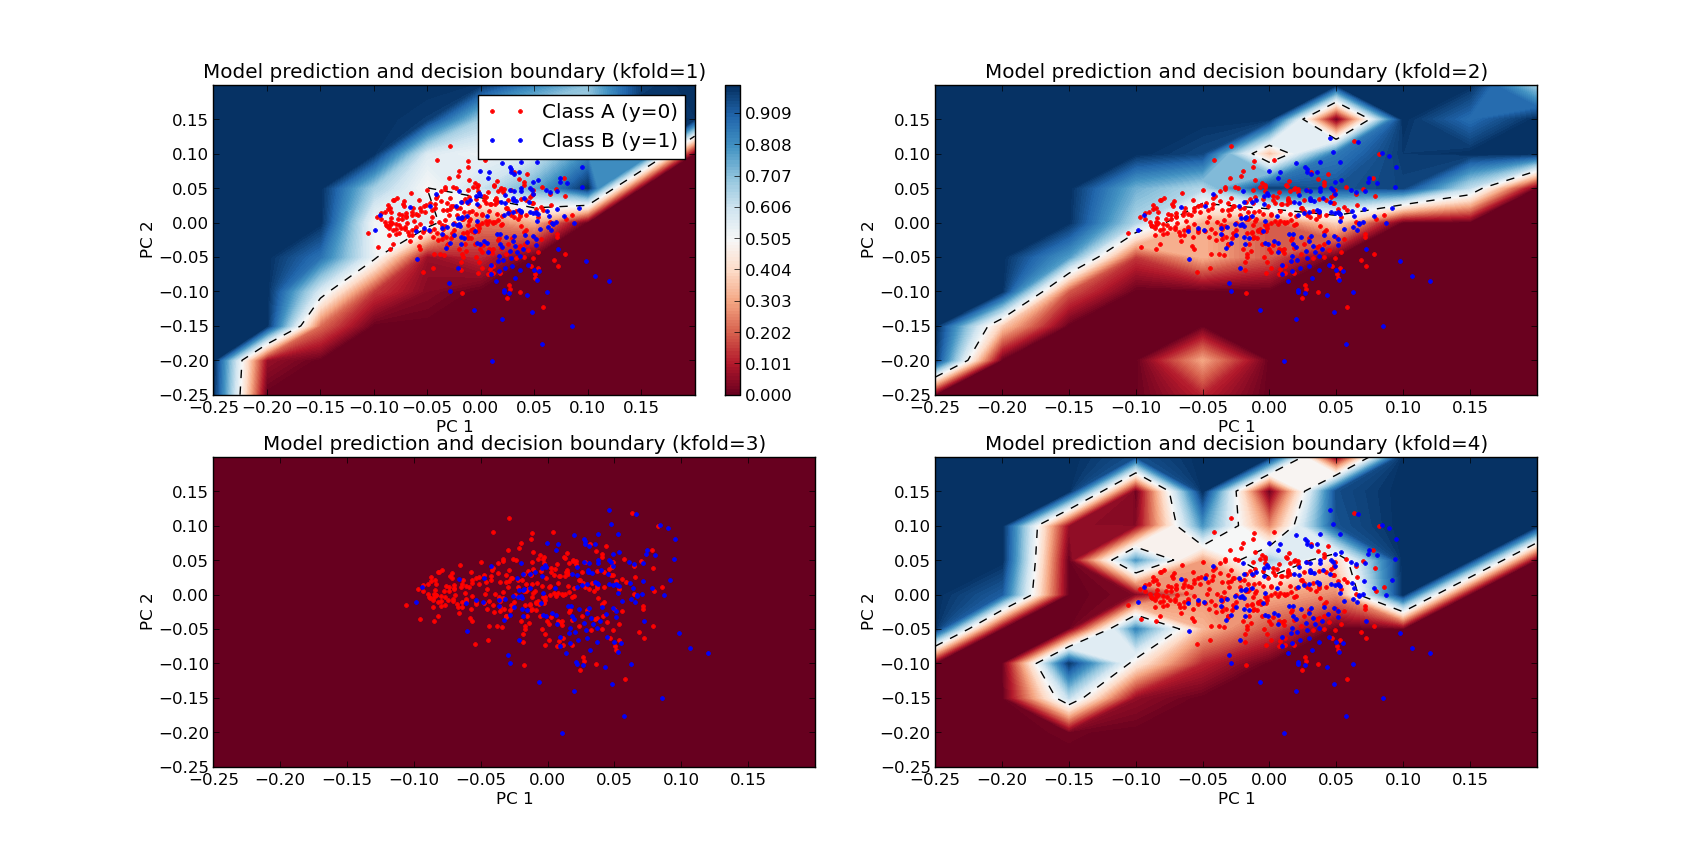
\includegraphics[width=15cm, keepaspectratio=true]{pictures/ann_2_4_230.png}
\vspace{-0.7cm}
\caption{\footnotesize }
\label{ann}
\end{figure}
Figure \ref{ann2} that we see below shows the learning curve of the above figure \ref{ann}, this shows how the training process improved over the number of epochs.
\begin{figure}[H]
\centering
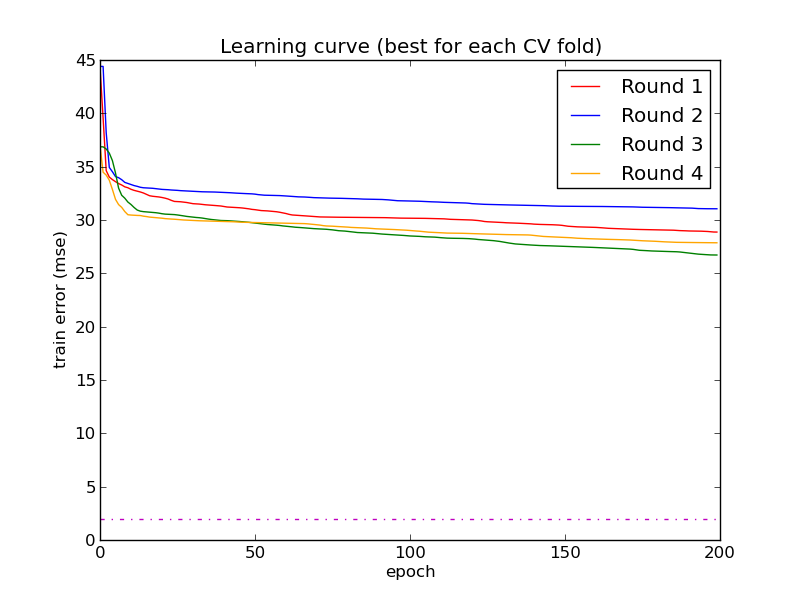
\includegraphics[width=7.5cm, keepaspectratio=true]{pictures/ann_21_4_230.png}
\vspace{-0.4cm}
\caption{\footnotesize }
\label{ann2}
\end{figure}